\documentclass[tikz,border=8pt]{standalone}
\usepackage{amsmath,amssymb}
\usetikzlibrary{arrows.meta,calc,angles,quotes}
\definecolor{TargetBlue}{HTML}{2364AA}
\definecolor{NuisanceOrange}{HTML}{E6862A}
\definecolor{EfficientGreen}{HTML}{278A64}
\definecolor{NeutralGray}{HTML}{68717C}
\begin{document}
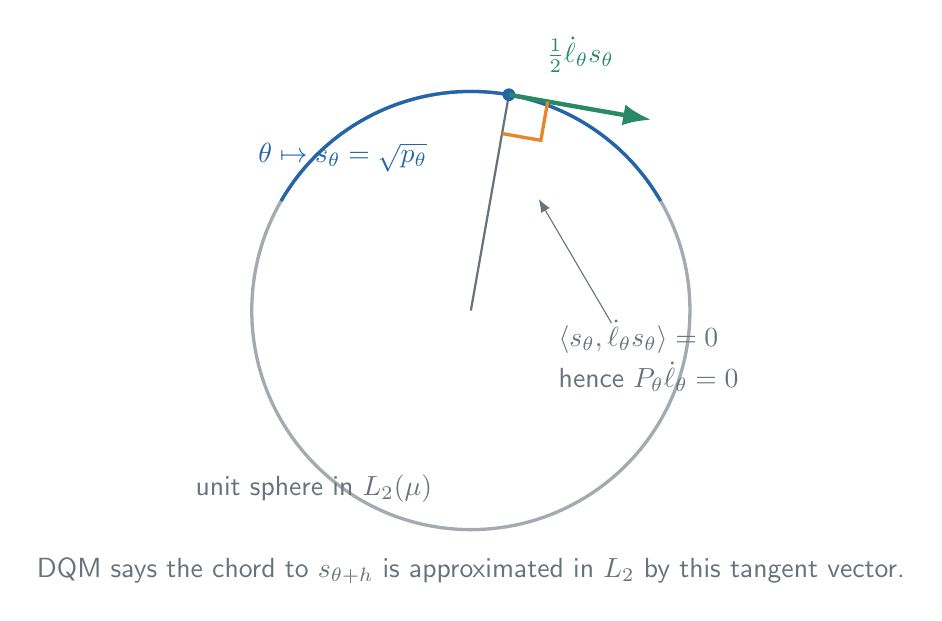
\begin{tikzpicture}[font=\sffamily, >=Latex, scale=1.05]
  \draw[NeutralGray!60, very thick] (0,0) circle (2.65);
  \node[text=NeutralGray] at (-1.9,-2.15) {unit sphere in $L_2(\mu)$};

  \draw[TargetBlue, very thick, domain=30:150, samples=100, smooth, variable=\t]
    plot ({2.65*cos(\t)},{2.65*sin(\t)});
  \node[text=TargetBlue] at (-1.55,1.85) {$\theta\mapsto s_\theta=\sqrt{p_\theta}$};

  \coordinate (O) at (0,0);
  \coordinate (P) at ({2.65*cos(80)},{2.65*sin(80)});
  \coordinate (T) at
    ({2.65*cos(80)+1.75*sin(80)},{2.65*sin(80)-1.75*cos(80)});
  \draw[NeutralGray, thick] (O) -- (P);
  \fill[TargetBlue] (P) circle (2.2pt);
  \draw[->, EfficientGreen, ultra thick] (P) -- (T)
    node[midway, above=3mm, text=EfficientGreen] {$\frac12\dot\ell_\theta s_\theta$};

  \pic[draw=NuisanceOrange, very thick, angle radius=5mm]
    {right angle=O--P--T};
  \node[align=left, text=NeutralGray] at (2.15,-0.55)
    {$\langle s_\theta,\dot\ell_\theta s_\theta\rangle=0$\\[1mm]
     hence $P_\theta\dot\ell_\theta=0$};
  \draw[->, NeutralGray] (1.7,-0.15) -- (0.82,1.35);

  \node[align=center, text=NeutralGray] at (0,-3.15)
    {DQM says the chord to $s_{\theta+h}$ is approximated in $L_2$ by this tangent vector.};
\end{tikzpicture}
\end{document}
